\documentclass[a4paper,12pt]{article}

%%% Работа с русским языком
\usepackage{cmap}					% поиск в PDF
\usepackage[T2A]{fontenc}			% кодировка
\usepackage[utf8]{inputenc}			% кодировка исходного текста
\usepackage[english,russian]{babel}	% локализация и переносы
\usepackage{indentfirst}			% отступ вначале параграфа


%%% Дополнительная работа с математикой
\usepackage{amsfonts,amssymb,amsthm,mathtools} % AMS
\usepackage{amsmath}
\usepackage{icomma} % "Умная" запятая: $0,2$ --- число, $0, 2$ --- перечисление

%% Номера формул
\mathtoolsset{showonlyrefs=true} % Показывать номера только у тех формул, на которые есть \eqref{} в тексте.

%% Шрифты
\usepackage{euscript}	 % Шрифт Евклид
\usepackage{mathrsfs} % Красивый матшрифт


%%% Работа с картинками
\usepackage{epstopdf}
\epstopdfsetup{update}
\usepackage{graphicx}  % Для вставки рисунков
\graphicspath{{images/}{images2/}}  % папки с картинками
\setlength\fboxsep{3pt} % Отступ рамки \fbox{} от рисунка
\setlength\fboxrule{1pt} % Толщина линий рамки \fbox{}
\usepackage{wrapfig} % Обтекание рисунков и таблиц текстом

%%% Работа с таблицами
\usepackage{array,tabularx,tabulary,booktabs} % Дополнительная работа с таблицами
\usepackage{longtable}  % Длинные таблицы
\usepackage{multirow} % Слияние строк в таблице


\usepackage{caption}
\captionsetup{labelsep=period}


%\title{Часть главы II}
%\author{Кравцов К.В.}
%\date{}

\begin{document}

%\maketitle

Пусть рис. \ref{1st} представляет положения Солнца $S$, Земли $T$ и Луны $L$, и пусть $\Theta$ есть центр тяжести Земли и Луны. Делаем следующие обозначения:

\begin{table}[h]
	\begin{center}
		\caption{Обозначения.}
		\begin{tabular}{|c|c|}

		\hline 
		Масса Солнца & $S$ \\ 
		\hline 
		>> Земли & $T$ \\ 
		\hline 
		>> Луны & $L$ \\ 
		\hline 
		
		\end{tabular}
	\end{center}
\end{table} 

Расстояние:

\[
	S\Theta = \rho;\text{ } ST = \rho_1;\text{ } SL = \rho_2;\text{ } TL = r
\]

тогда будет:

\begin{equation}\label{eq:eqfirst}
	\begin{aligned}
		T\Theta &= r_1 = \cfrac{L}{T+L} \cdot r \\
		L\Theta &= r_2 = \cfrac{T}{T+L} \text{ } r	
	\end{aligned}
\end{equation}


%	\begin{equation}\label{eq:eqfirst}
%		T\Theta &= r_1 = \cfrac{L}{T+L} \cdot r \\
%		L\Theta &= r_2 = \cfrac{T}{T+L} \text{ } r	
%	\end{equation}


\begin{wrapfigure}{r}{0.5\linewidth}
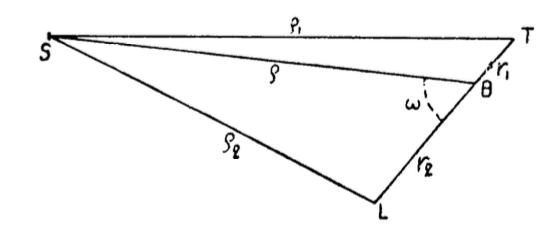
\includegraphics[width=0.9\linewidth]{21}
\caption{}\label{1st}
\end{wrapfigure} Составим теперь выражения ускорений, которые эти тела сообщают друг другу.

Солнце $S$ сообщает ускорения:


\[
	\begin{aligned}
		&\text{Земле: } &&f \cdot \cfrac{S}{\rho_1^2} &&\text{ по направлению} &TS \\
		&\text{Луне: } &&f \cdot \cfrac{S}{\rho_2^2} &&\text{ >> } \quad\qquad \text{  >>   } &LS
	\end{aligned}
\]


вследствие чего точка $\Theta$ имеет ускорения:


\[
	\begin{aligned}
		&\cfrac{T}{T+L} \cdot f \cdot \cfrac{S}{\rho_1^2} &&\text{ по направлению, параллельному} &TS \\
		&\cfrac{L}{T+L} \cdot f \cdot \cfrac{S}{\rho_2^2} &&\text{ >> } \quad\qquad \text{  >>   } \qquad\qquad \text{  >>   } &LS
	\end{aligned}
\]


Ускорения Солнца, происходящие от притяжения Земли и Луны, соответственно, суть:


\[
	\begin{aligned}
		&f \cdot \cfrac{T}{\rho_1^2} &&\text{ по направлению} &ST \\
		&f \cdot \cfrac{L}{\rho_2^2} &&\text{ >> } \quad\qquad \text{  >>   } &SL
	\end{aligned}
\]


поэтому ускорения точки $\Theta$ относительно точки $S$ будут:


\[
	\begin{aligned}
		\omega_1 &= f \cdot \cfrac{(S+T+L)}{T+L} \cdot \cfrac{T}{\rho_1^2} &&\text{ по направлению параллельно} &TS \\
		\omega_1 &= f \cdot \cfrac{S+T+L}{T+L} \cdot \cfrac{L}{\rho_2^2} &&\text{ >> } \quad\qquad \text{  >>   } \  \qquad\qquad \text{  >>   } &LS
	\end{aligned}
\]

Разлагая эти ускорения, соответственно, по направлениям $\Theta S$ и $\Theta L$, получим, как легко видеть из подобия показанных на рис. \ref{2nd} и \ref{3rd} треугольников:

\[
	\begin{aligned}
		\omega_1^{'} &= \omega_1 \cdot \cfrac{\rho}{\rho_1} &&\text{ по направлению} &\Theta S \\
		\omega_1^{''} &= \omega_1 \cdot \cfrac{r_1}{\rho_1} &&\text{ >> } \quad\qquad \text{  >>   } &\Theta L \\
		\omega_2^{'} &= \omega_2 \cdot \cfrac{\rho}{\rho_2} &&\text{ >> } \quad\qquad \text{  >>   } &\Theta S \\
		\omega_2^{''} &= \omega_2 \cdot \cfrac{r_2}{\rho_2} &&\text{ >> } \quad\qquad \text{  >>   } &L \Theta
	\end{aligned}
\]

\begin{figure}[bhtp]
\centering
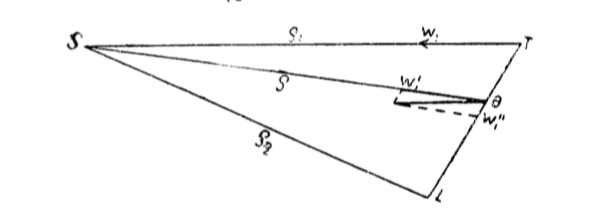
\includegraphics{22}
\caption{}\label{2nd}
\end{figure}


получим для ускорений точки $\Theta$ слагающие:


\[
	\begin{aligned}
		W_1 &= \omega_1^{'} + \omega_2^{'} = f \cdot \cfrac{S+T+L}{T+L} \cdot \left[ T \cdot \cfrac{\rho}{\rho_1^3} + L \cdot \cfrac{\rho}{\rho_2^3} \right] \text{ по } \Theta S \\	
		W_2 &= \omega_1^{''} - \omega_2^{''} = f \cdot \cfrac{S+T+L}{T+L} \cdot \left[ T \cdot \cfrac{r_1}{\rho_1^3} - L \cdot \cfrac{r_2}{\rho_2^3} \right] \text{ по } \Theta L
	\end{aligned}	
\]


\begin{figure}[bhtp]
\centering
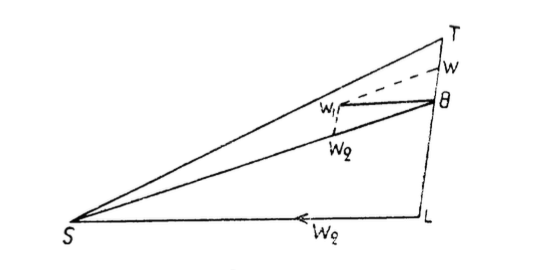
\includegraphics{23}
\caption{}\label{3rd}
\end{figure}


Заменив $r_1$ и $r_2$ их выражениями \eqref{eq:eqfirst}, имеем:


\[
	\begin{aligned}
		W_1 &= f \cdot \cfrac{S+T+L}{T+L} \cdot \rho \cdot \left[ \cfrac{T}{\rho_1^3} + \cfrac{L}{\rho_2^3} \right] \text{ по направлению } \Theta S \\	
		W_2 &= f \cdot \cfrac{S+T+L}{(T+L)^2} \cdot T \cdot L \cdot r \cdot \left[ \cfrac{1}{\rho_1^3} - \cfrac{1}{\rho_2^3} \right] \text{ по направлению } \Theta L
	\end{aligned}	
\]


Но


\[
	\begin{aligned}
		\rho_1^2 &= \rho^2 + 2 \rho \cdot \cfrac{L}{T+L} \cdot r \cos \omega + \left( \cfrac{L}{T+L} \cdot r \right) ^2 \\
		\rho_2^2 &= \rho^2 - 2 \rho \cdot \cfrac{T}{T+L} \quad r \cos \omega + \left( \cfrac{T}{T+L} \text{ }r \right) ^2 \\
	\end{aligned}
\]


следовательно:


\[
	\begin{aligned}
		\cfrac{1}{\rho_1^3} = \cfrac{1}{\rho^3} \left[ 1 + 3 \, \cfrac{L}{T+L} \, \cos \omega + \left( \cfrac{L}{T+L} \text{ }r \right) ^2 \left( - \cfrac{3}{2} + \cfrac{15}{2} \cos ^2 \omega \right) + \cdots \right] \\
		\cfrac{1}{\rho_2^3} = \cfrac{1}{\rho^3} \left[ 1 + 3 \, \cfrac{T}{T+L} \, \cos \omega + \left( \cfrac{T}{T+L} \text{ }r \right) ^2 \left( - \cfrac{3}{2} + \cfrac{15}{2} \cos ^2 \omega \right) + \cdots \right]
	\end{aligned}
\]


Подставляя эти выражения, имеем:


\[
	\begin{aligned}
		W_1 &= f \cdot \cfrac{S+T+L}{\rho^2} \left[ 1 + \cfrac{T \cdot L}{(T+L)^2} \cdot \cfrac{r^2}{\rho^2} \left( - \cfrac{3}{2} + \cfrac{15}{2} \cos ^2 \omega \right) + \cdots \right] \\
		W_2 &= f \cdot \cfrac{S+T+L}{\rho^2} \left[ - 3 \cdot \cfrac{T \cdot L}{(T+L)^2} \cdot \cfrac{r^2}{\rho^2} \cos \omega + \cdots \right]
	\end{aligned}
\]


Но отношения


\[
	\cfrac{L}{T+L} \approx \cfrac{1}{80} ; \quad \cfrac{r}{\rho} \approx \cfrac{1}{400} ; \quad \left( \cfrac{r}{\rho} \right) ^2 = \cfrac{1}{160000}
\]


поэтому будет


\[
	\cfrac{T \cdot L}{T+L} \cdot \cfrac{r^2}{\rho^2} \approx \cfrac{1}{12800000}
\]	


и члены, содержащие этот множитель, могут быть отброшены, так что будет:


\[
	\begin{aligned}
		W_1 &= f \cdot \cfrac{S+T+L}{\rho^2} \text{ по направлению } \Theta S \\
		W_2 &= 0 \text{ по направлению } \Theta L 
	\end{aligned}
\]


Отсюда следует, что точка $\Theta$ движется вокруг Солнца по эллиптической орбите по законам Кеплера.

Рассмотрим теперь ускорение Луны по отношению к Земле, для чего к ускорениям, сообщаемым Луне Солнцем и Землею, надо присовокупить ускорение, равное и противоположенное ускорению Земли, происходящему от действия Солнца и Луны. Поступив подобно предыдущему, получим:


\[
	\begin{aligned}
		f \cdot \cfrac{T+L}{r^2} &+ f \cdot S \left[ \cfrac{r_2}{\rho_2^3} + \cfrac{r_1}{\rho_1^3} \right] \text{ по направлению } L \Theta \\
		f \, \cdot \, &S \cdot \rho \left[ \cfrac{1}{\rho_2^3} - \cfrac{1}{\rho_1^3} \right] \text{параллельно } \Theta S
	\end{aligned}
\]


положим:

\[
	T + L = \mu ; \text{ } S = M
\]


\listoffigures
\listoftables
 

\end{document}
